\documentclass[a4paper, 11pt]{article}

\usepackage{graphicx}

\begin{document}
\section{Grammar structure}
\subsection{Problem introduction}

NOTE: Here we assume that Rascal/MPS are already introduced


In this section we will introduce the problem of communicating the core "structure" of the textually defined grammar to a projectional editor. The core "structure" referenced here refers most closely to the abstract syntax tree of the grammar in question, i.e the non-terminals and their production rules, stripped of any layout information and literals. For example, lets take the production as shown in Figure~\ref{fig:startSyntax}. At this stage, all we are concerned with is:

\begin{itemize}
	\item There is a non-terminal (Program).
	\item With a labeled production rule (prog).
	\item The rule contains a single "Declarations" non-terminal labeled "decls".
	\item The rule contains 0 to n "Statement" non-terminals labeled "body".
\end{itemize}

We can visualize this structure as a tree as in figure~\ref{fig:startSyntaxAST}. Note that any purely visual information, such as the literals ("begin", ";" and "end") are lost. These will be handled under the Editor section of this thesis.


\begin{figure}[h]
	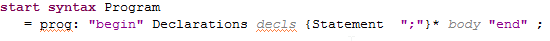
\includegraphics[width=\linewidth]{images/StartSyntax2.png}
	\caption{Textual grammar production rule}
	\label{fig:startSyntax}
\end{figure}

\begin{figure}[h]
	\centering
	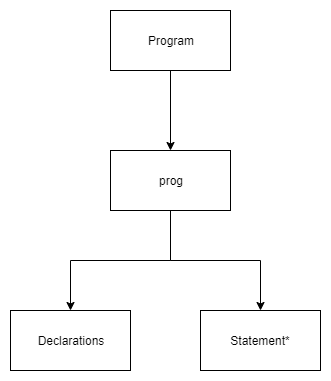
\includegraphics[scale=0.5]{images/AST.png}
	\caption{AST visualized}
	\label{fig:startSyntaxAST}
\end{figure}

Now that we have a clear idea of what elements of the textual grammar we want to recreate in the projectional editor, we can start defining the sub-problems of how to do so. These goals will be as follows:

\begin{itemize}
	\item[1] Extract the AST from the textual grammar definition.
	\item[2] Transfer this AST to the projectional editor.
	\item[3] Recreate the projectional model using the AST data.
\end{itemize}

We will now describe how our solution solve each of these defined sub-problems and how these put together solve the overall problem of recreating the core "strucure" of the grammar as a projectional model. First we will show a general overview of the solution and it's parts. Then we will take a closer look at each part in itself and show how it solves one of the sub-problems. 

\subsection{General overview}

The general architectural overview of the solution in context of the Rascal and MPS worlds is presented in Figure~\ref{fig:world}. There are two main components, which exchange information through an intermediary format. 

\begin{figure}[h]
	\centering
	\includegraphics[scale=0.4]{images/World_Definition.png}
	\caption{Rascal2MPS architecture and context}
	\label{fig:world}
\end{figure}

\begin{itemize}
	\item Rascal2XML generates an the AST representation of a given Rascal grammar and outputs it as a XML file. 
	\item XML2MPS takes a XML file representing a Rascal grammar AST, creates a new MPS Language and populates the Structure Aspect of said MPS Language by constructing Interfaces and Concepts based on the given AST.  
\end{itemize}

Both parts are implemented within their own respective world: Rascal2XML consists of multiple Rascal modules and is thus called from the Eclipse editor. XML2MPS is implemented as multiple MPS solutions and a MPS plugin, and is correspondingly called from within MPS. The approach is therefore a two-step process: First one exports the XML-version of an AST representing a Rascal grammar. Next, one opens MPS with the XML2MPS plugin loaded and imports this XML file. 
\\\\ 
An alternative to this two-step approach would have been to implement the solution in such a manner that the abstract syntax tree can be communicated directly between both worlds, without the need for a file-based intermediary format. Such a solution was considered and tested early on in the project. This solution took advantage of the fact that Rascal itself is implemented in Java, and MPS has native support for importing and calling Java JAR files. The idea was to implement functions within Rascal, create a JAR of the entire Rascal runtime environment, including the implemented methods for creating an AST from a Rascal grammar file, and call these functions from within MPS. This would bypass the need for an external file-based data storage, as it would give us direct access to Rascal data types and functions. Unfortunately, this approach ran into technical problems.
\\\\
NOTE: TODO More detailed explanation of the technical problem 
\\\\
Solving these problems would have required extensive research into both Rascal and MPS internal code. In the end, there were enough advantages to the two-step approach using a file-based intermediary format that it was chosen as for our solution. More about the choice of XML as our intermediary file-based format and the potential advantages a file-based intermediary format can bring us is presented in the "Intermediary format" section of this chapter.
\\\\
Next we will take a closer look at each of the components of the solution and how these relate to the given sub-problems.
\subsection{Intermediary format}

\subsection{Rascal2XML}
First we will explore the problem of generating an abstract syntax tree from a given Rascal grammar file and storing this data in our file-based intermediary format, in this case XML. 
\\\\
To generate the abstract syntax tree of a given grammar file, we can reuse existing Rascal functionality in the \# operator. In Rascal, calling #NonTerminal where NonTerminal is the name of some Rascal syntax construct will generate a tree-like structure representing the grammar following this non-terminal. Thus calling this operator on the root of the grammar will generate a kind of "dummy" parse tree containing information about all the different alternatives for each non-terminal encountered recursively from the starting rule. In Rascal, starting symbols of a grammar are signified by the "start" keyword before a "syntax" declaration, as can be seen in Figure~\ref{fig:startSyntax}. In this case, we can obtain the representative parse tree of this grammar using "\#Program". 
\\\\
This Rascal Tree structure however is quite large contains much more information than we require for our core "structure" as described in the introduction to this chapter. It contains for example layout information, literals and  lexical definitions. To extract only the information we require we perform a top-down tree walk over the generated tree, filtering out the core structure, using pattern matching on the desired structures. There is one important distinction made by the algorithm here, namely between non-terminals and their production rules and lexicals. Lexicals in Rascal are a way for the language engineer to constrain user input using regular expressions. Exactly how lexicals are handled by Rascal2XML and XML2MPS in discussed in a later section. For now, it suffices to say that they are registered during the tree walk, since they appear in child nodes of production rules. 
\\\\
Besides selecting the required data from the Rascal parse tree, there is also another purpose to the tree walk. While we are doing th tree walk, we simultaneously construct DOM nodes using the Rascal standard DOM library. 
The constructed DOM encodes the tree that is to be stored in XML format and later used by the XML2MPS component. It thus must contain any relevant information we wish to move between the worlds. 
\\\\
On the core structure level, the DOM is quite simple:
\begin{itemize}
	\item There is a single top-level root node
	\item Containing 0..n "nonterminal" nodes.
	\item Each "nonterminal" node has:
	\begin{itemize}
		\item A "name" child node with the non-terminal name
		\item 0..n "production" nodes; one for each production rule of the non-terminal.
		\item Each "production" node contains:
		\begin{itemize}
			\item  A "name" child node with the production rule label
			\item 0..n "arg" nodes containing the references to other grammar structure.
			\item Each of which contains:
			\begin{itemize}
				\item "name" child node containing the reference label
				\item "type" child node containing the reference non-terminal name
				\item "card" child node containing the cardinality of the reference, either 1..1, 0..n or 1..n.
			\end{itemize}
		\end{itemize}
	\end{itemize}
\end{itemize}

For example, if we take the our production rule in Figure~\ref{fig:startSyntax} and put it through the algorithm, we end up with a corresponding XML file as shown in Figure~\ref{fig:XML}. This is all the information we need to start creating a MPS Language and populate the Structure Aspect in the XML2MPS component.

\begin{figure}[h]
	\centering
	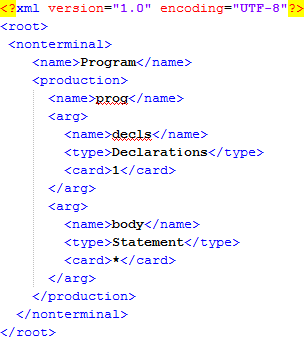
\includegraphics[scale=0.7]{images/StartSyntaxXML.png}
	\caption{XML representation of a Rascal grammar rule structure}
	\label{fig:XML}
\end{figure}


\subsection{XML2MPS}
The next task will be to take the XML file generated by Rascal2XML, create a new MPS Language and populate the Structure Aspect of said MPS Language. To this end we must decide how to map the Rascal non-terminal and production rules to MPS model components. 
\subsection{Lexicals}
\subsection{Limitations}
NOTE: This subsection might be better as its own chapter instead.
There are several limitations to the current approach that place restrictions on the source grammar. 
The current restrictions are:

\begin{itemize}
	\item All production rules must be labeled. This concerns the label of a production rule, for example the "prog" for the production rule shown in Figure~\ref{fig:startSyntax}. Rascal does not actually require this label to be present. A production rule declaration as in Figure~\ref{fig:UL} is perfectly valid. However, when creating our MPS Language Structure Aspect, we use this label as name for the constructed MPS Concept. One approach to this problem is for there to be some automated renaming scheme for when the rule is unlabeled. However this run into several other problems: Concept names must be unique and users will use the concept name to select the element in the projectional editor. Thus the name must be descriptive; having several versions of "dummy" does not tell the user what element they are actually inserting. Renaming also becomes a problem in one of the other major problems we are trying to solve, namely the program importing, where name matching is used to determine the structure of the model. In the end, we chose to restrict the source grammar to require labeled production rules, since this does not alter the expressiveness of the grammar in any way while allowing us to create 
	\item All non-terminal and production label names must be unique. MPS does not allow duplicate names of Concepts and Interfaces. Since the non-terminal and production label names are directly mapped to Interfaces and Concepts, these must also be unique. An alternative approach would be to have a renaming scheme in the case of duplicate names. However, how to do so  in a way that is both automated while remaining descriptive enough for use in the projectional editor is not a trivial problem. Thus for our solution, we chose to restrict the source grammar.  
	\item Lexicals must be either from 
	
\end{itemize}

\begin{figure}[h]
	\centering
	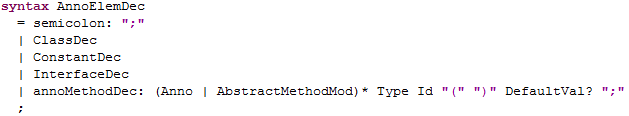
\includegraphics[width=\textwidth]{images/UnlabeledProduction.png}
	\caption{Syntax declaration using unlabeled production rules}
	\label{fig:UL}
\end{figure}

\end{document}